\chapter{Transparent Healthcare}

\section{Information seeking}

% Cancer information is important
When diagnosed with cancer patients and their family members lives change radically. They receive treatments and have to make choices with serious consequences. Such diseases and treatments are complex, but should be understood before decisions are made. Patients and their family members should be provided with intelligible and up to date information on the stage of disease, treatment options and complementary therapies \cite{butow_dynamics_1997,cassileth_information_1980}. Involving cancer patients in decision-making on their pathways improves their satisfaction and quality of life \cite{sheabudgell_information_2014}. On the contrary, patients who need health information but experience difficulties are at risk of experiencing poorer psychosocial health \cite{arora_barriers_2002}.

Carefully designed communication interventions have an impact on the patient's knowledge and recall, patient satisfaction and their ability to manage the symptoms \cite{johnson_effects_1982,hack_feasibility_1999,mohide_randomised_1996,mcpherson_effective_2001}. Some evidence indicates that preparing patients ahead of time for the clinical visit by providing practical information has a beneficial effect \cite{huchcroft_testing_1984,cegala_patient_2003}.

The demonstrated benefits of information seeking for cancer patients, coupled with increases in information availability, underscore the importance of monitoring patient information seeking experiences over time \cite{finney_rutten_cancer-related_2016}.

Communication facilitates the patients involvement in their own healthcare, reduces distress, improves adherence to, and compliance with, treatment regimens and increases the patient's sense of control \cite{viswanath_science_2005}.

Considerable research shows that medically related education interventions are most effective when they are tailored to patients' individual needs. While this matter is relevant to all patient communication skills training, it may be especially relevant to cancer patients \cite{cegala_patient_2003}.

% The communications revolution
The way we communicate and interact with information has drastically changed in the past years. We see more and more data from different sources generated each day, combined with a proliferation in the number of information delivery platforms. A large number of people now have smartphones that allow them to access information and the time or place they want. Consequently, we notice several shifts in how people access and use information. First, mass audience is fragmented into more closely aligned smaller groups who share common characteristics and interests. Additionally, there has been a shift in audience media use patterns, with the growth of the online audience far outpacing those for other media. It is now easy to access technical reports, scientific articles, and consensus guidelines, as they are available on many websites open to anyone with an Internet access. While these materials may not always be intended for a mainstream audience, their availability offers opportunities for access and interpretation by different groups \cite{viswanath_communications_2012}.

% Growing quantity of information available
The quantity of cancer information available in the media and on the internet has been growing rapidly over the past decades \cite{viswanath_science_2005,viswanath_communications_2012}, changing how patients interact with providers based on advice and input from peers and family members. Communication has been found to play a central role in cancer prevention and control. It can provide information on cancer prevention, monitor lifestyles and health behaviors, promote participatory decision making during cancer detection, diagnosis, and treatment, and foster quality of life during survivorship or end of life  \cite{viswanath_communications_2012}.

% Patients are looking for information
As a matter of fact, patients are often seeking information during their pathways. In the United States of America, a survey from the Health Information National Trends (HINTS) \cite{hesse_trust_2005} measured online health activities, levels of trust, and source preference for 6,369 people. They showed that 63.7\% of the online population in the US looked for health information for themselves or others. Although an increasing number of patients were looking for information online, physicians remained the most trusted source of information.

% How do patients get their information ?
A Canadian study surveyed patients attending appointments at follow-up cancer clinics in Calgary, Alberta \cite{sheabudgell_information_2014} between 2011 and 2012. They approached 648 patients and obtained responses from 411 one of them. The study aimed at: identifying information needs of patients when meeting their physician for a follow-up; listing patients preferences on how to receive information. Here are the results they gathered regarding information seeking patterns. The most frequently reported source of information was the Internet (57.4\%); health provider (32.6\%), brochures or pamphlets (25.1\%), and cancer organizations (24.3\%). The most frequently reported types of information sought included information about a specific type of cancer (43.1\%), treatment or cures for cancer (29.4\%), prognosis or recovery from cancer (29.0\%), and prevention of cancer (27.0\%). The least frequently reported types of cancer information sought included where to get medical care (3.4\%), paying for medical care or insurance (4.6\%), and cancer organizations (5.4\%). Regarding trust, the physician or health care provider was largely the most trusted source of information, followed by Internet, and family and friends. The least trusted sources of information included radio, newspaper, and television.

% Patients are not always satisfied with the amount of information they receive
Despite actively looking for information, there is increasing evidence that patients with cancer require more information about their disease and its consequences than they receive \cite{mcpherson_effective_2001}.

Moreover, studies shown that patients are often not satisfied with the information they receive, or forget or misunderstand the information conveyed \cite{ley_communicating_1988,hogbin_getting_1989}. The interaction with their physician has also been cited as a major cause of dissatisfaction \cite{stewart_effective_1995,bartlett_effects_1984} at all stages of illness \cite{higginson_palliative_1990}. Patients reported insufficient time spent on communication during the clinical encounter and physicians inability to keep up with the most current information and advances in cancer care \cite{anderson_impact_2003}.

% Internet to help patients
As a result of this dissatisfaction with information and communication with their physician, patients have started to search for health information and resources on the internet \cite{chen_impact_2001,pereira_internet_2000,ziebland_how_2004,dolce_internet_2011}. Research has been conveyed to better understand the relationship between physicians and cancer patients, and how they used the internet as a source of health information \cite{dolce_internet_2011}. An online questionnaire was administered to participants of cancer-related communities hosted by the Association of Cancer Online Resources (ACOR). As a result, 488 participants shared their personal experiences with accessing health online resources. Several participants reported not receiving the most up-to-date cancer information from their physician. Diagnostic failures in which symptoms had been undiagnosed, incorrectly diagnosed, or dismissed by their healthcare provider also happened for some patients. This is especially true for rare cancers and unusual side effects. Patients who encountered physicians with lack of clinical expertise consequently turned to the Internet to fill the information gap. For instance, participants who experienced a lack of informational support related to procedures found blogs and testimonies online that helped them to know what to expect from a physical and emotional perspective. Sometimes, for rare diseases, physicians can benefit from patients looking from additional information online, as it may bring additional knowledge to them, and even change their plans for care. Aware patients can also challenge their physicians by asking meaningful questions and participate in the tailoring of their treatment plans. Finally, online communities allowed patients to identify physicians with a proven track record in cancer care. They endorsed care providers who took the time to answer questions, as well as specialists from major cancer centers, that brought superior care which led to better outcome.

The increased usage of the Internet by cancer patients thus puts new demands on health care professionals. Patients need advice about how to find reliable and credible web sites and also help with authenticating and interpreting the information they find \cite{carlsson_cancer_2009}.

% Disparities in information accessibility
However, while mass media communications can be an important source of health information, research found social disparities in health knowledge that may be related to media use. Indeed, cancer-related health communications seems to be patterned by race, ethnicity, language, and social class. The benefits of health information are not equally distributed across socially distinct groups in the United States \cite{viswanath_race_2011}. Moreover, a lower likelihood of cancer information seeking was also observed among those with lower education levels, lower income and greater ages \cite{finney_rutten_cancer-related_2016}.

% Importance of quality in surgery
\cite{glaser_surgeon_2019}
\cite{bonati_surgeon_2021}
\cite{renzulli_learning_2005}
\cite{renzulli_influence_2006}
\cite{read_surgeon_2002}
\cite{mcdermott_surgeon_2013}
\cite{yen_surgeon_2014}
\cite{nietz_quality_2020}

% \section{Healthcare-Network web application}

% \begin{figure}[H]
%     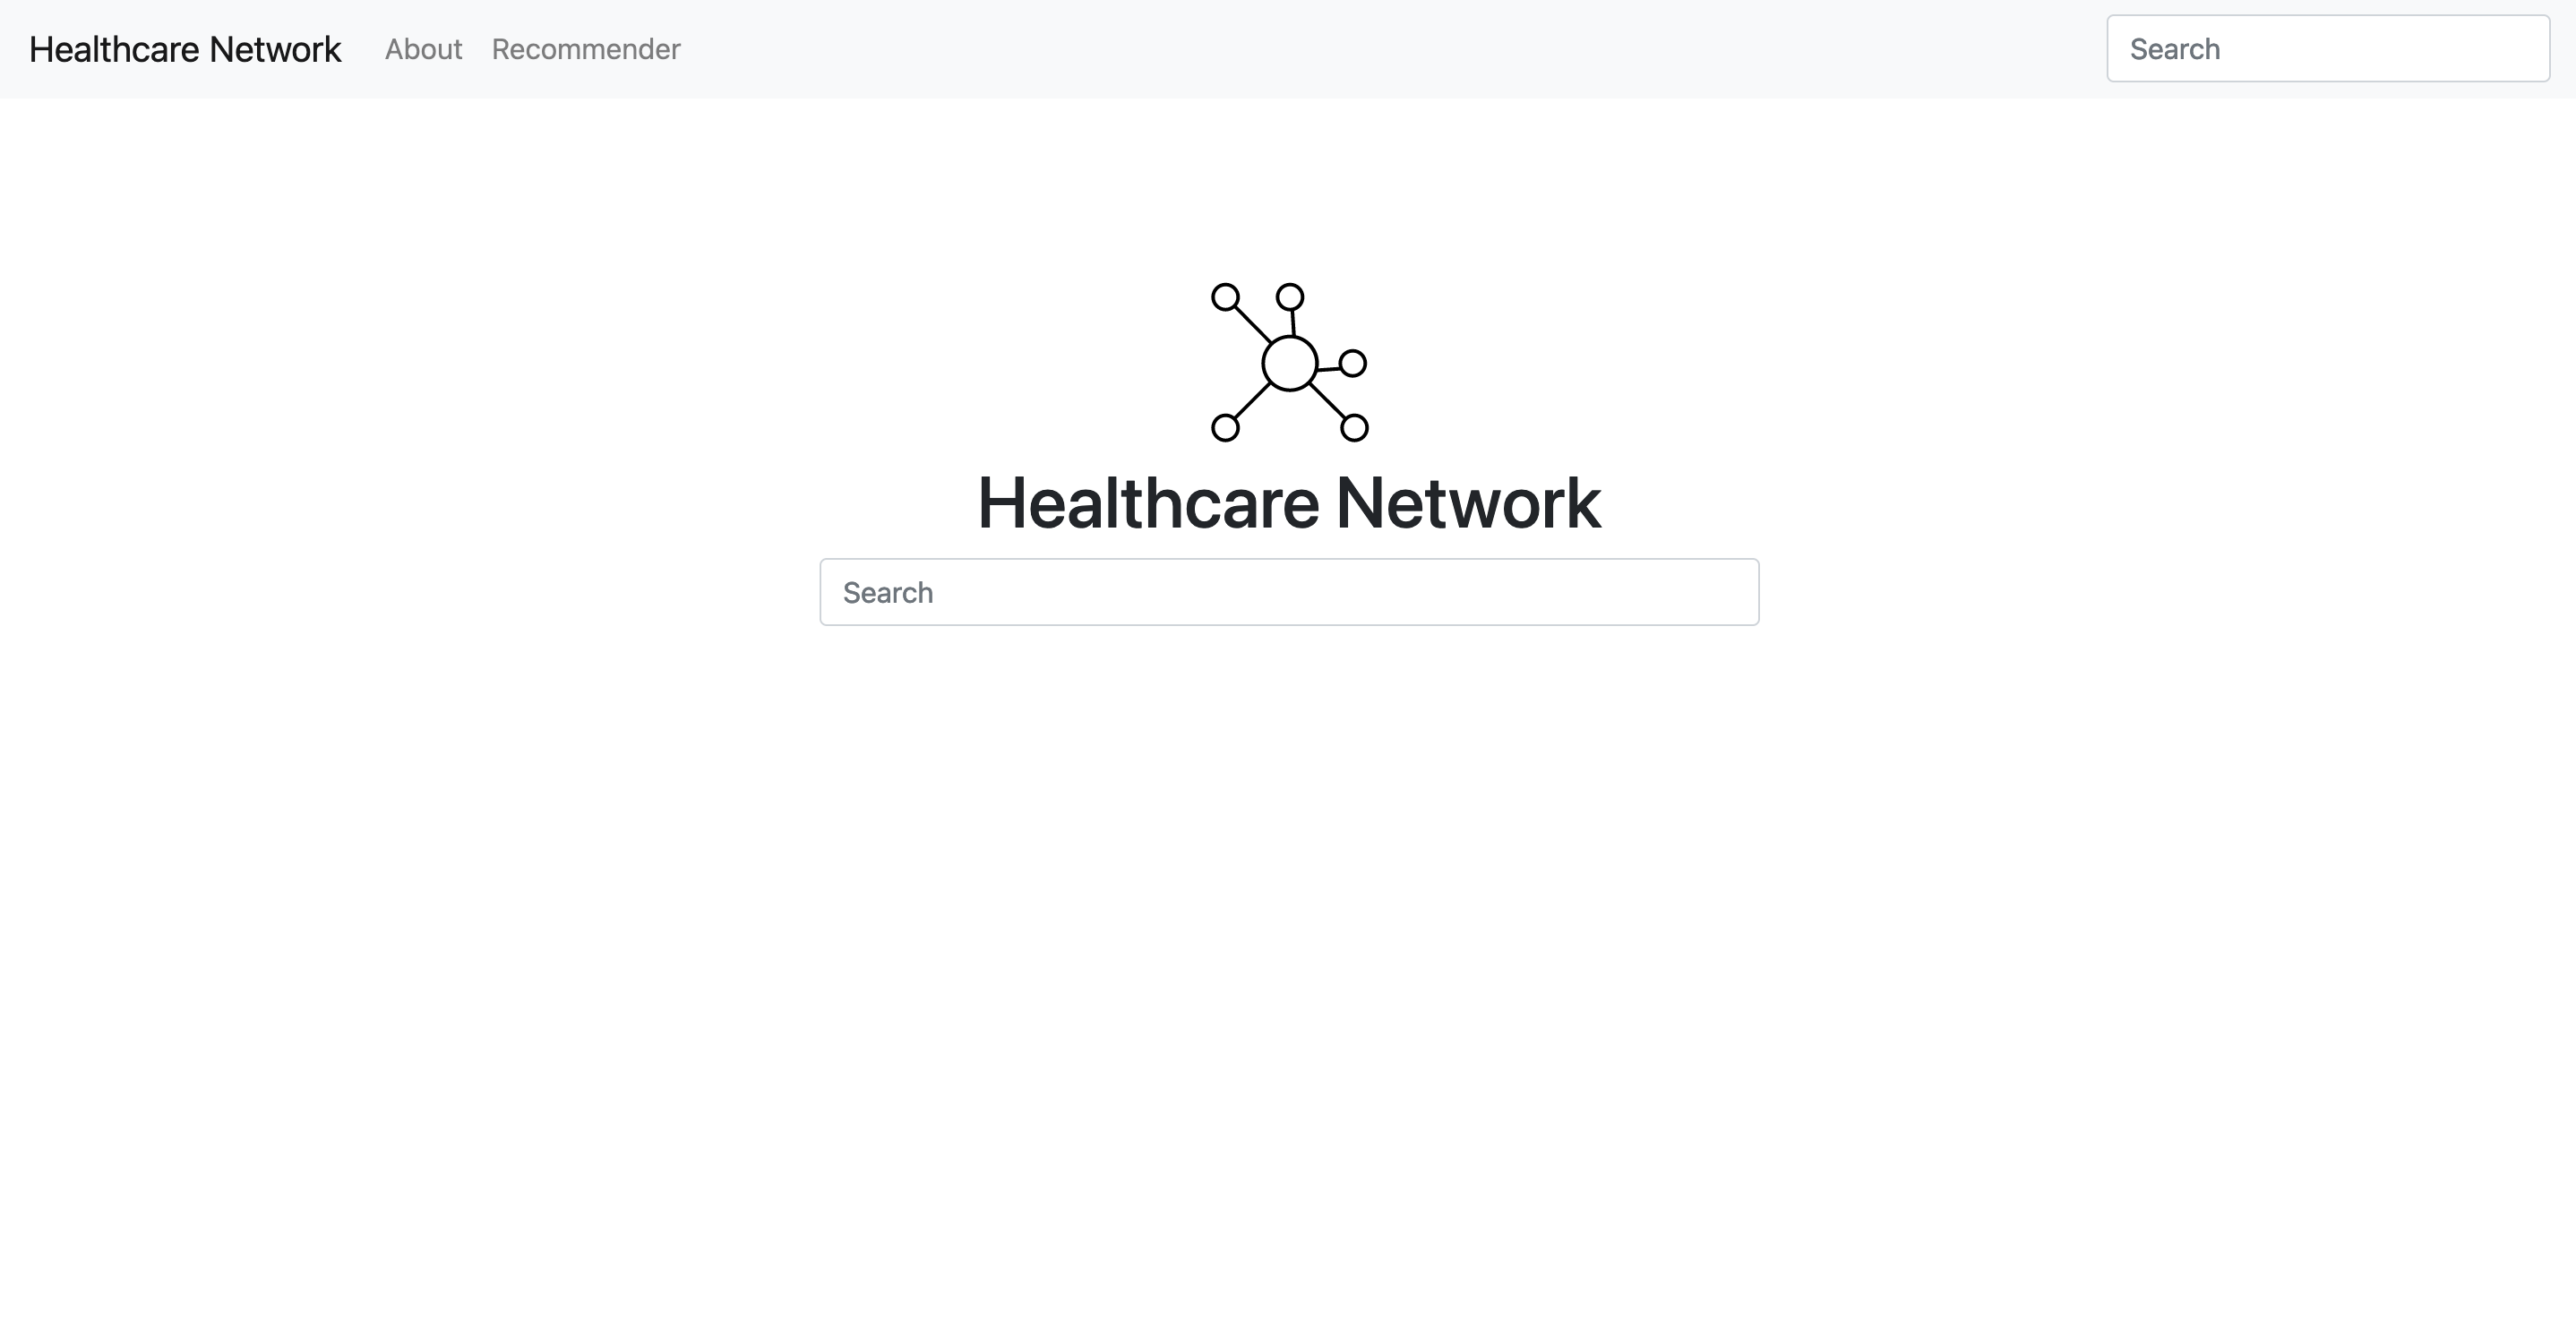
\includegraphics[width=0.7\textwidth]{images/healthcare-network/home.png}
%     \centering
%     \caption{
%         \textbf{Healthcare-Network: homepage.} A minimalist page with a search bar allowing to find hospitals based on their name, category, or location.
%     }
%     \label{fig:hn-home}
% \end{figure}


% \begin{figure}[H]
%     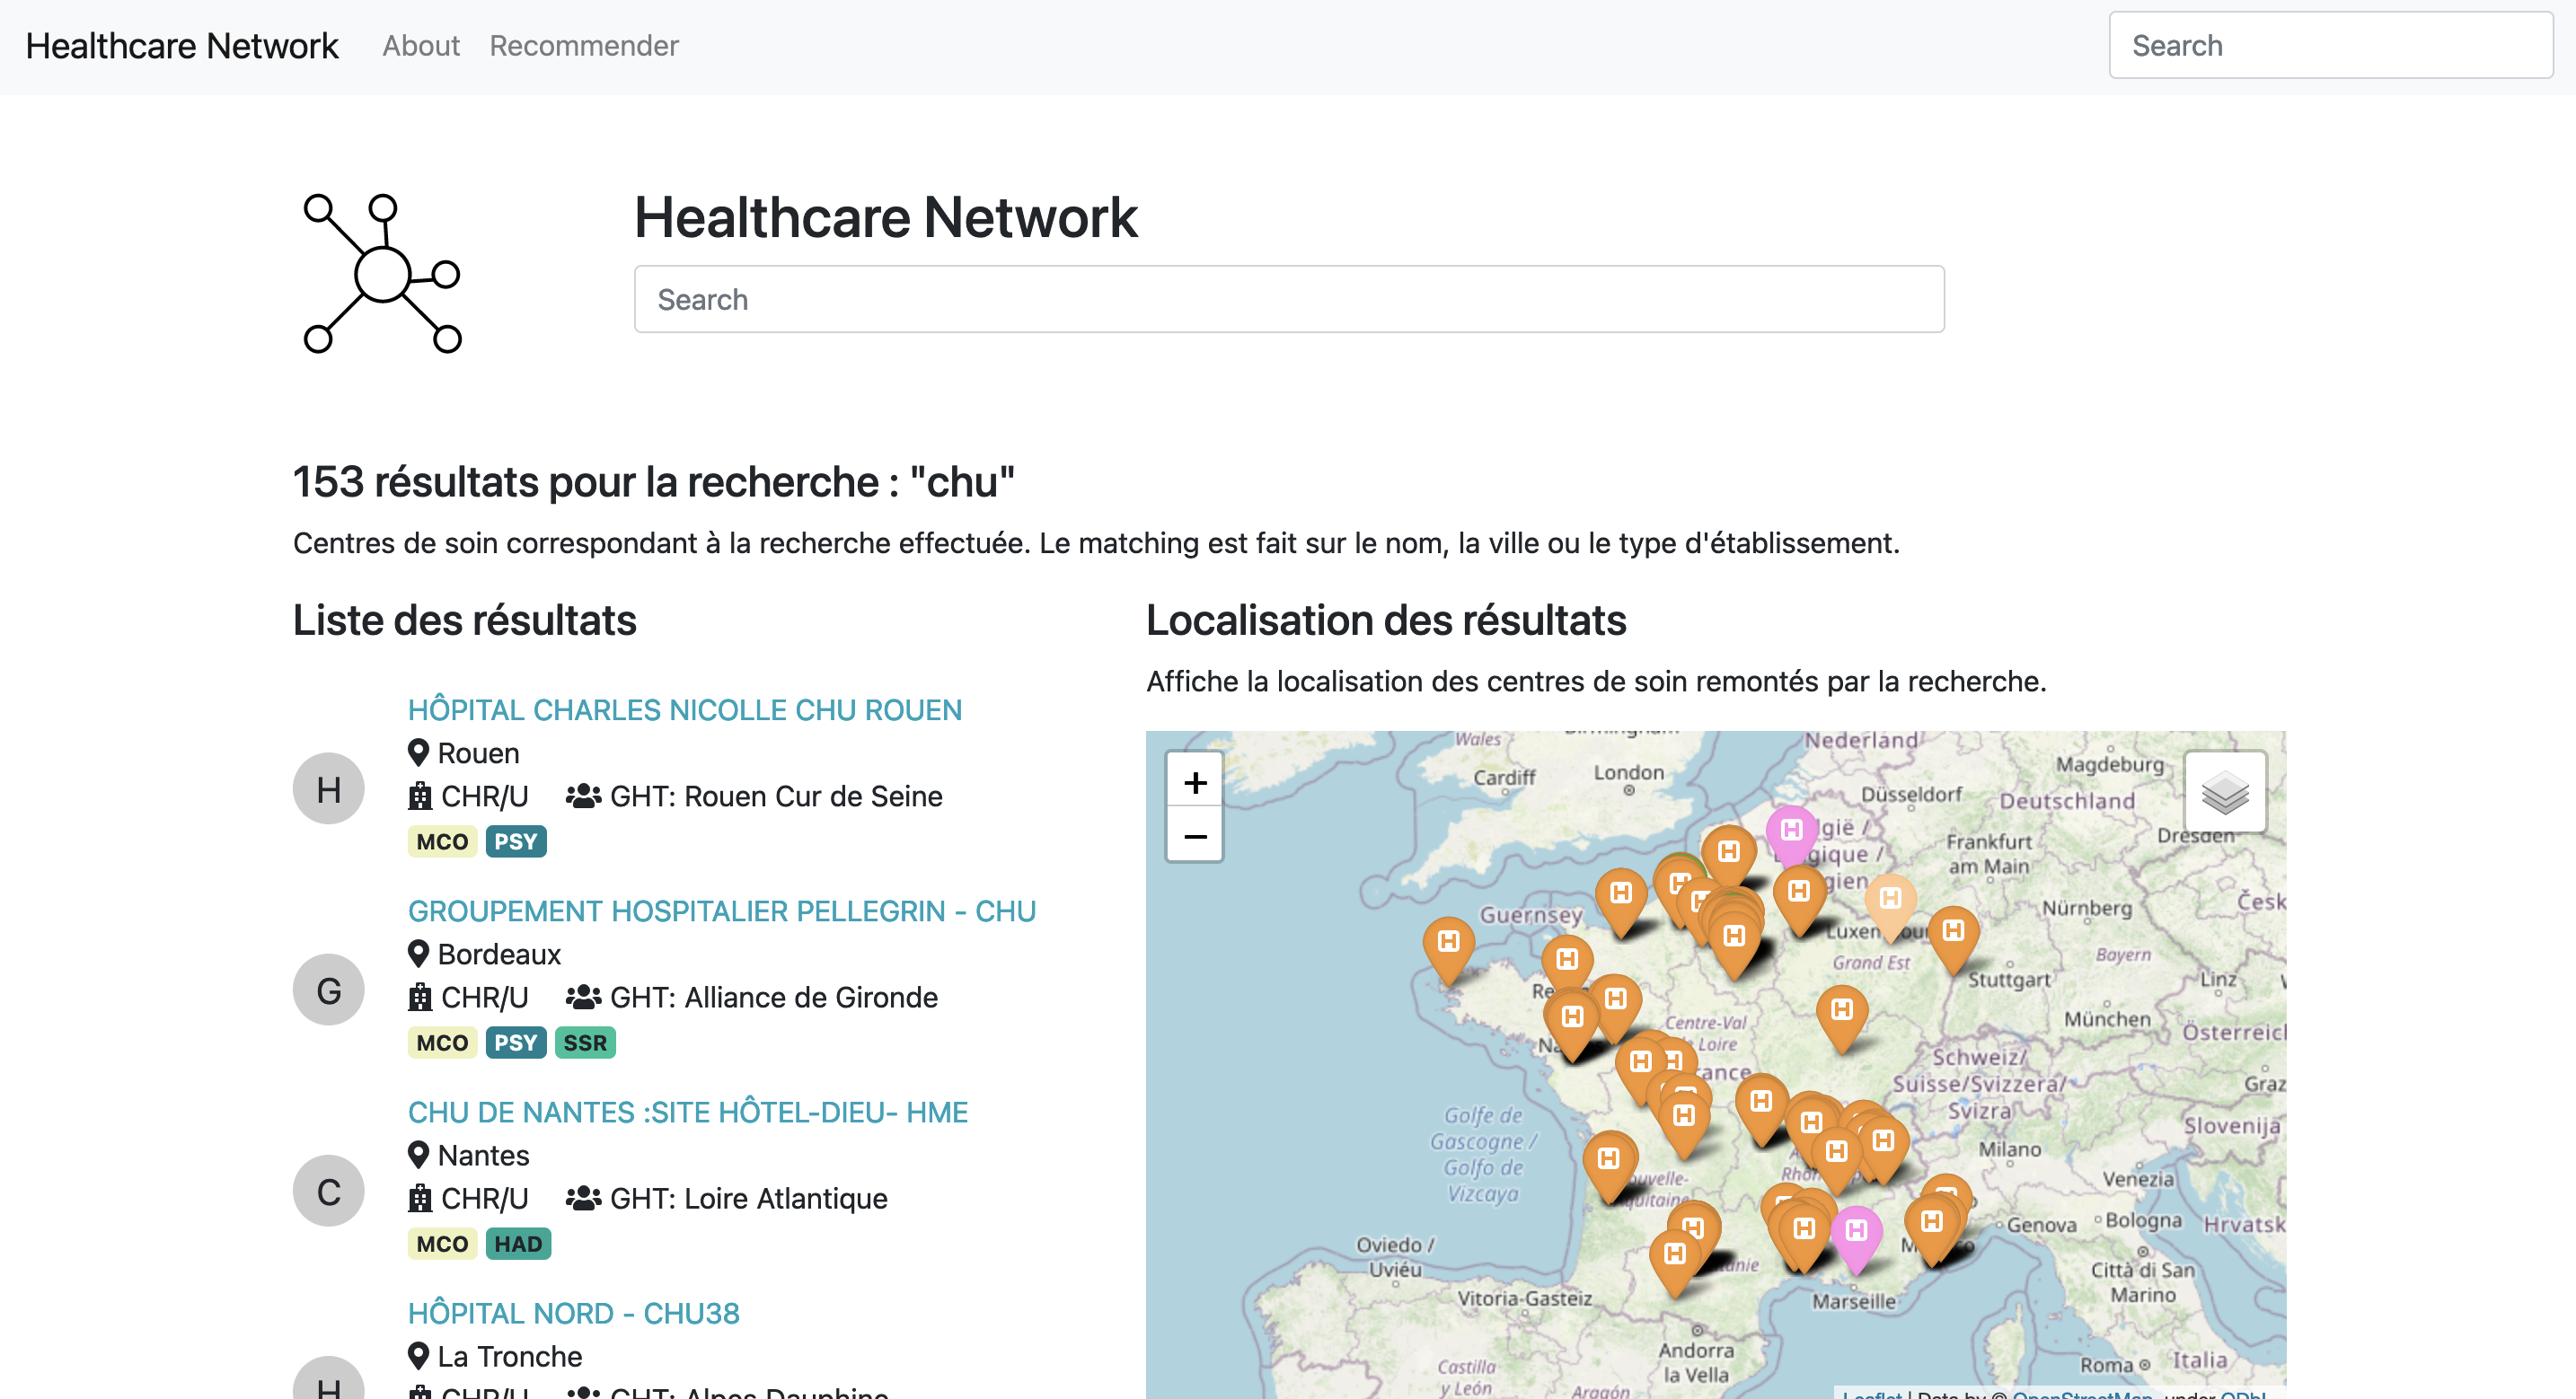
\includegraphics[width=0.7\textwidth]{images/healthcare-network/search.png}
%     \centering
%     \caption{
%         \textbf{Healthcare-Network: search results.} The list of retrieved hospitals and their details is displayed, as their position on a map. This query shows all the \ac{chru} hospitals in metropolitan France.
%     }
%     \label{fig:hn-search}
% \end{figure}


% \begin{figure}[H]
%     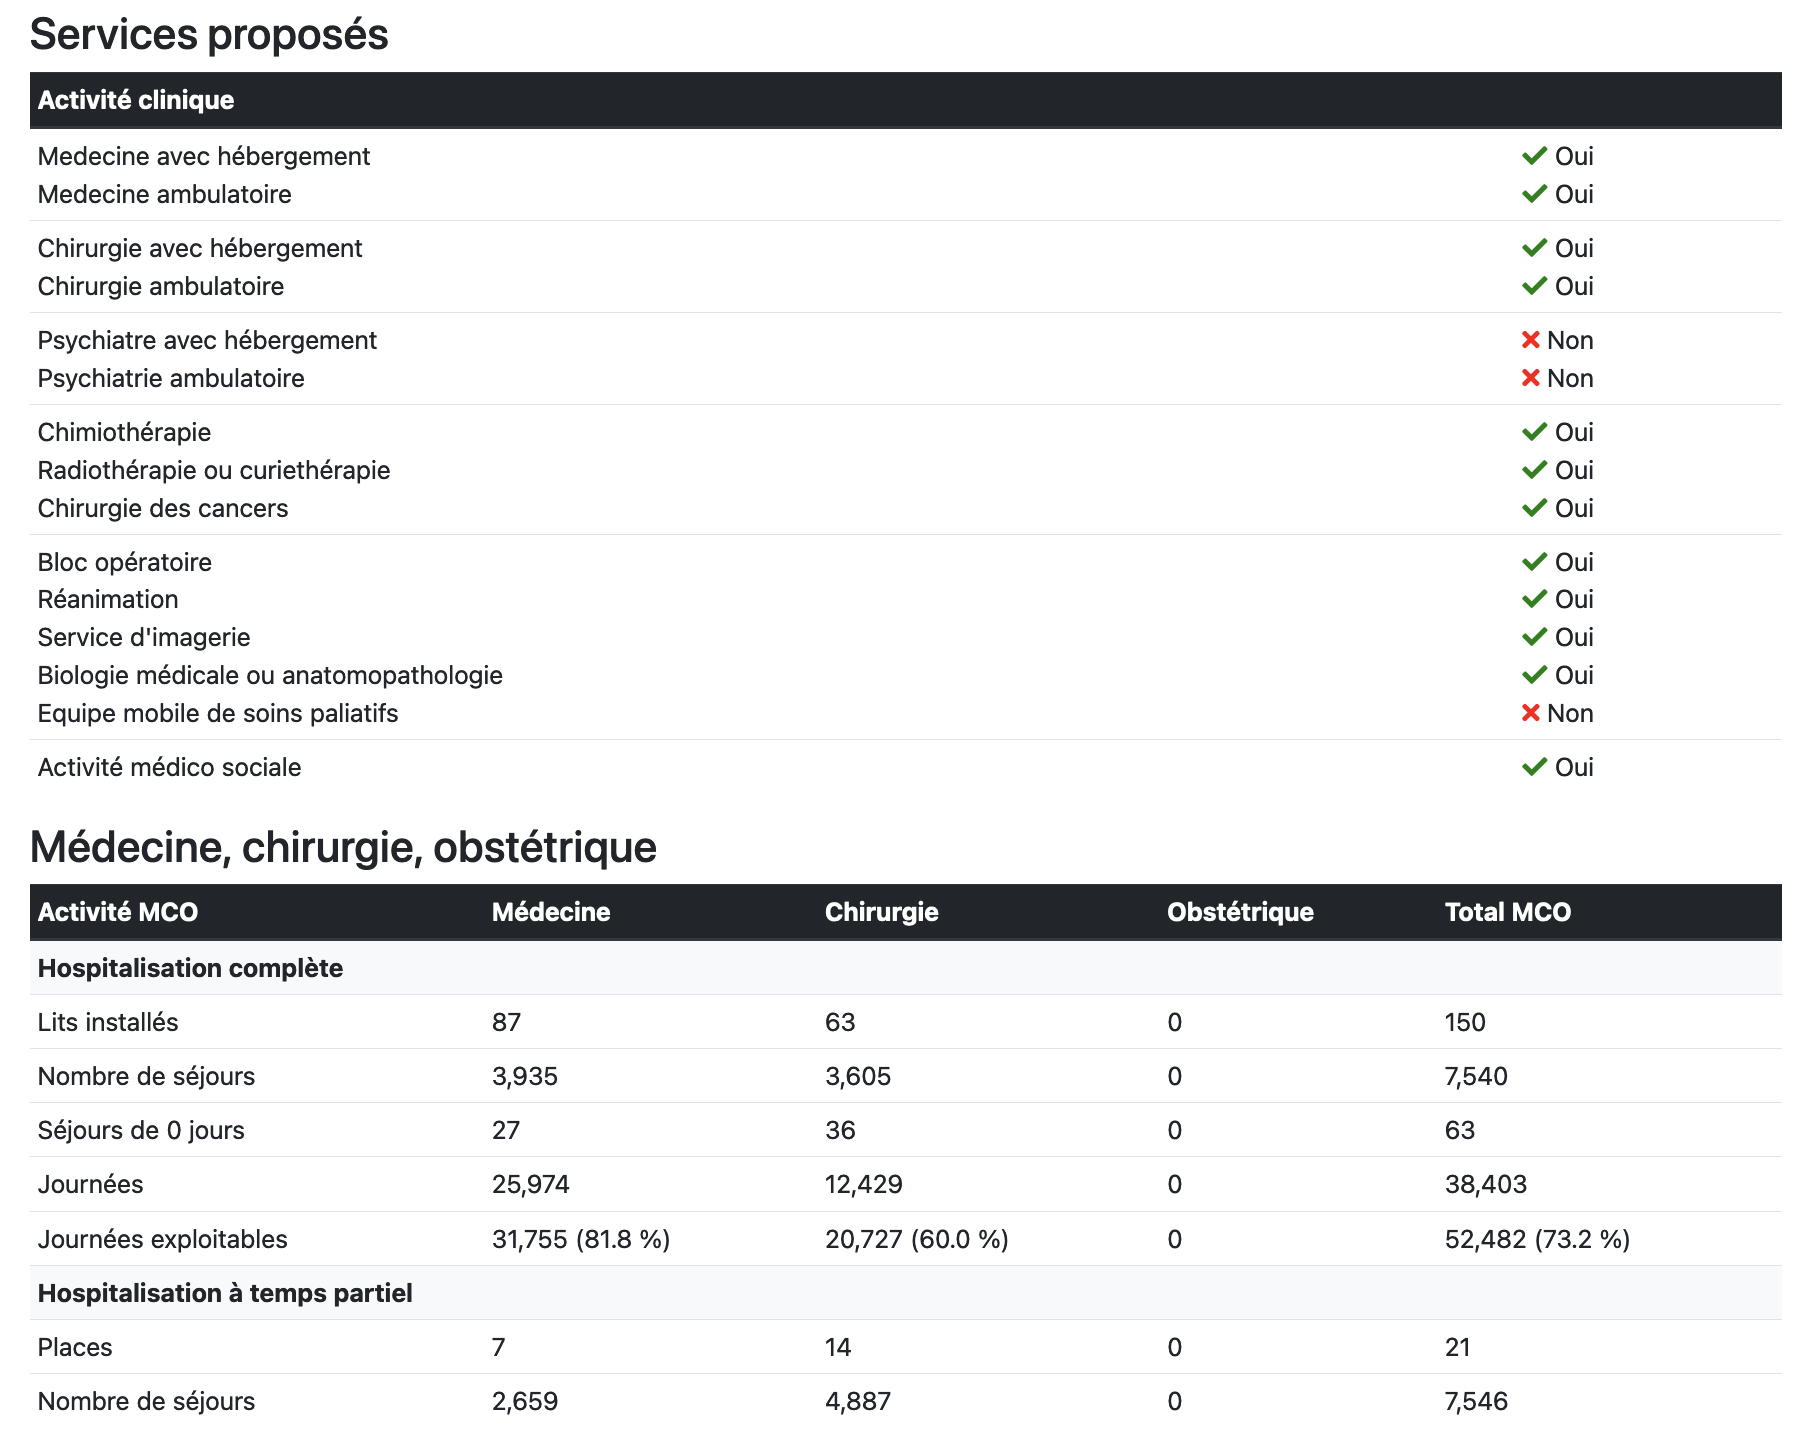
\includegraphics[width=0.7\textwidth]{images/healthcare-network/curie-services.png}
%     \centering
%     \caption{
%         \textbf{Healthcare-Network: description of health services offered, and statistics on \ac{mco} activity for Institut Curie Paris hospital.}
%     }
%     \label{fig:hn-curie-services}
% \end{figure}


% \begin{figure}[H]
%     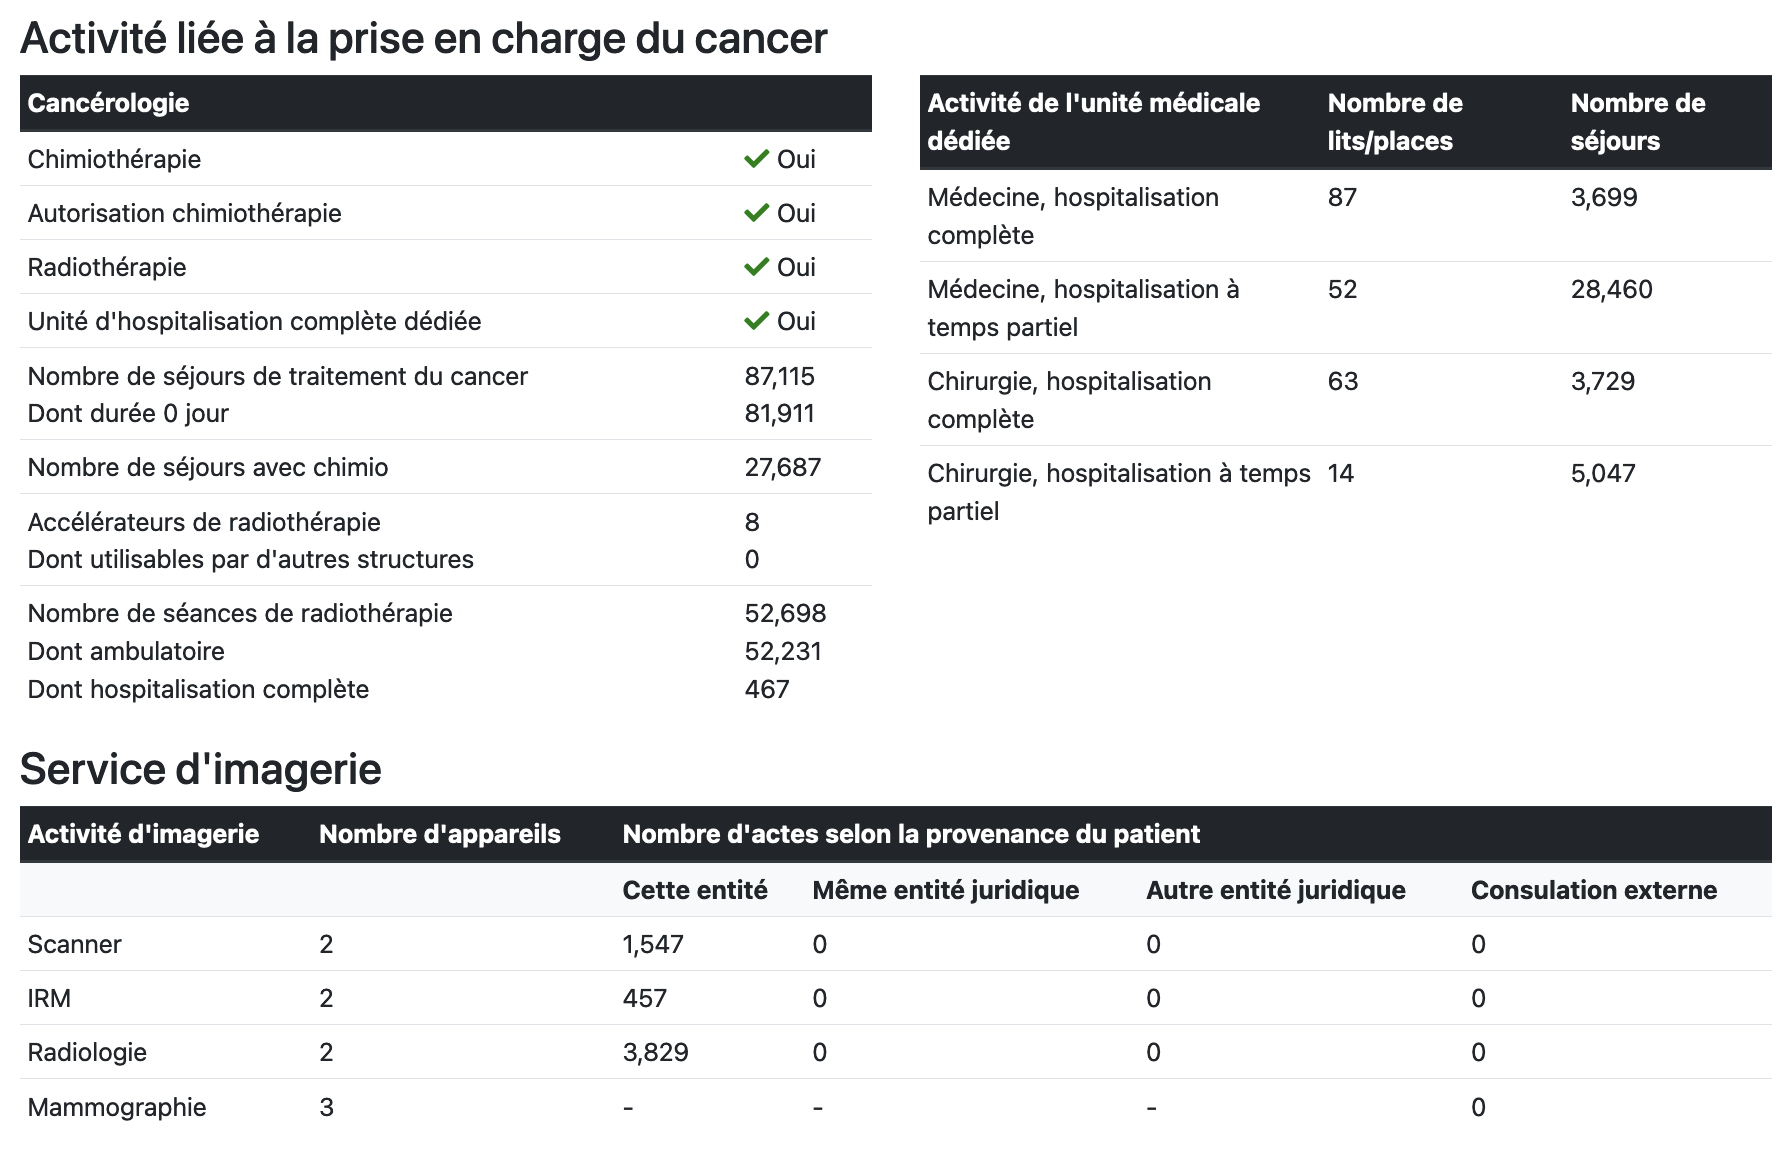
\includegraphics[width=0.7\textwidth]{images/healthcare-network/curie-cancero.png}
%     \centering
%     \caption{
%         \textbf{Healthcare-Network: description of oncology activity for Institut Curie Paris hospital.}
%     }
%     \label{fig:hn-curie-cancero}
% \end{figure}


% \begin{figure}[H]
%     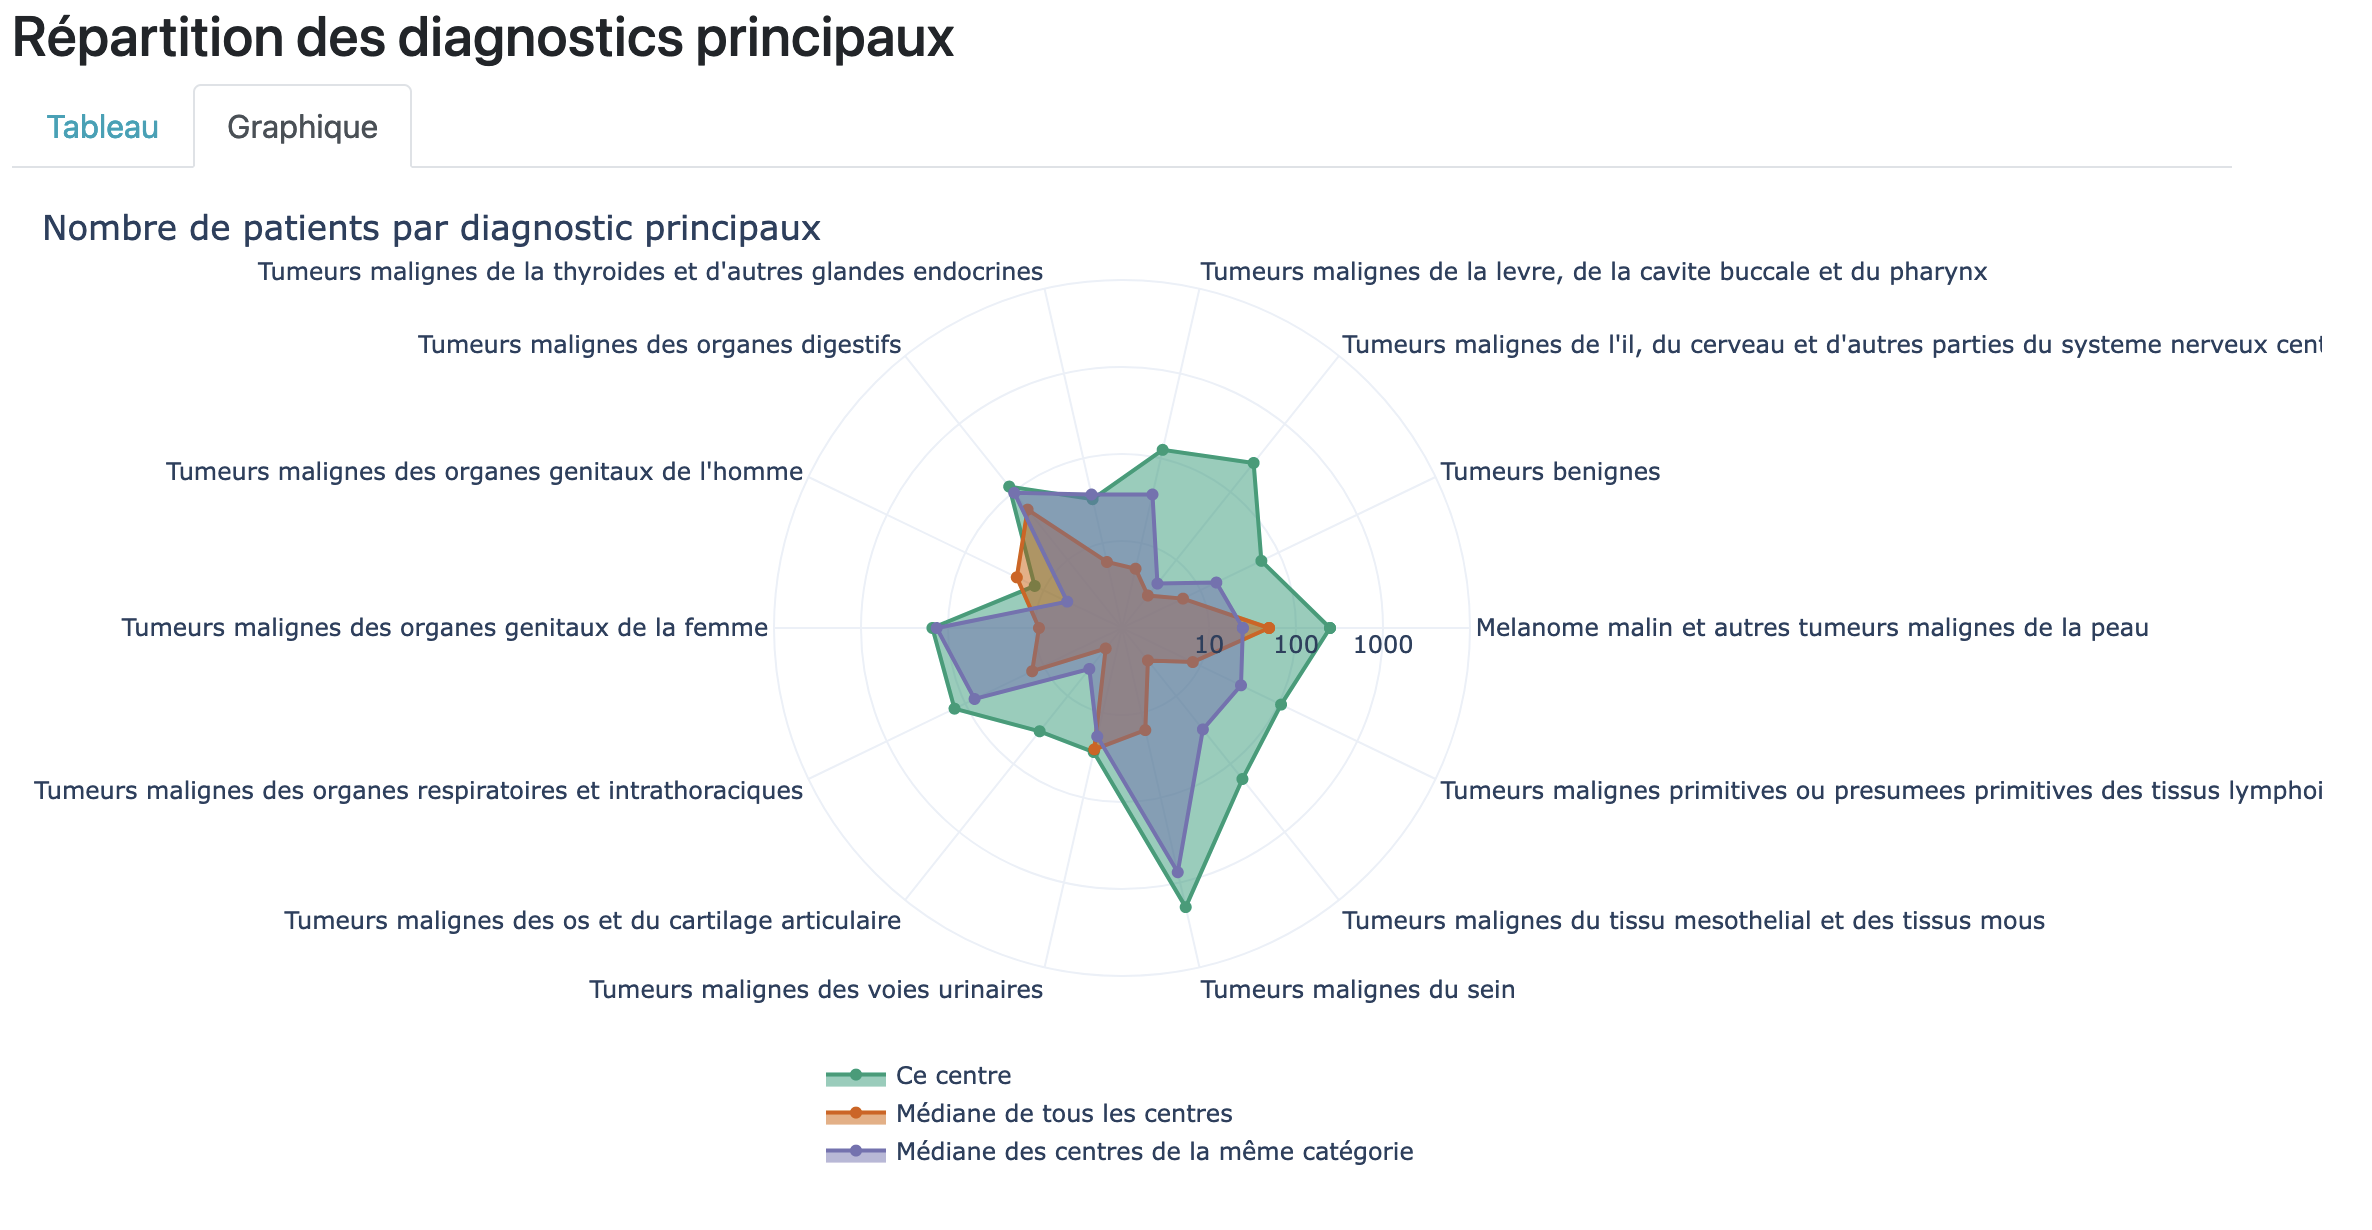
\includegraphics[width=0.7\textwidth]{images/healthcare-network/curie-dp.png}
%     \centering
%     \caption{
%         \textbf{Healthcare-Network: number of patients per cancer related diagnosis for Institut Curie Paris hospital.} Comparison with the median statistics from hospitals within the same category (\ac{clcc}) and overall median.
%     }
%     \label{fig:hn-curie-dp}
% \end{figure}


% \begin{figure}[H]
%     \includegraphics[width=0.7\textwidth]{images/healthcare-network/curie-co-occ.png}
%     \centering
%     \caption{
%         \textbf{Healthcare-Network: map of the hospitals that have the most co-occurrences with Institut Curie Paris.} Co-occurrences between two hospitals are defined as the number of patients who visited both hospitals during their care pathways. To illustrate facility attractiveness, municipalities are colored by the number of inhabitants who visited the Institut Curie Paris hospital.
%     }
%     \label{fig:hn-curie-co-occ}
% \end{figure}


% \begin{figure}[H]
%     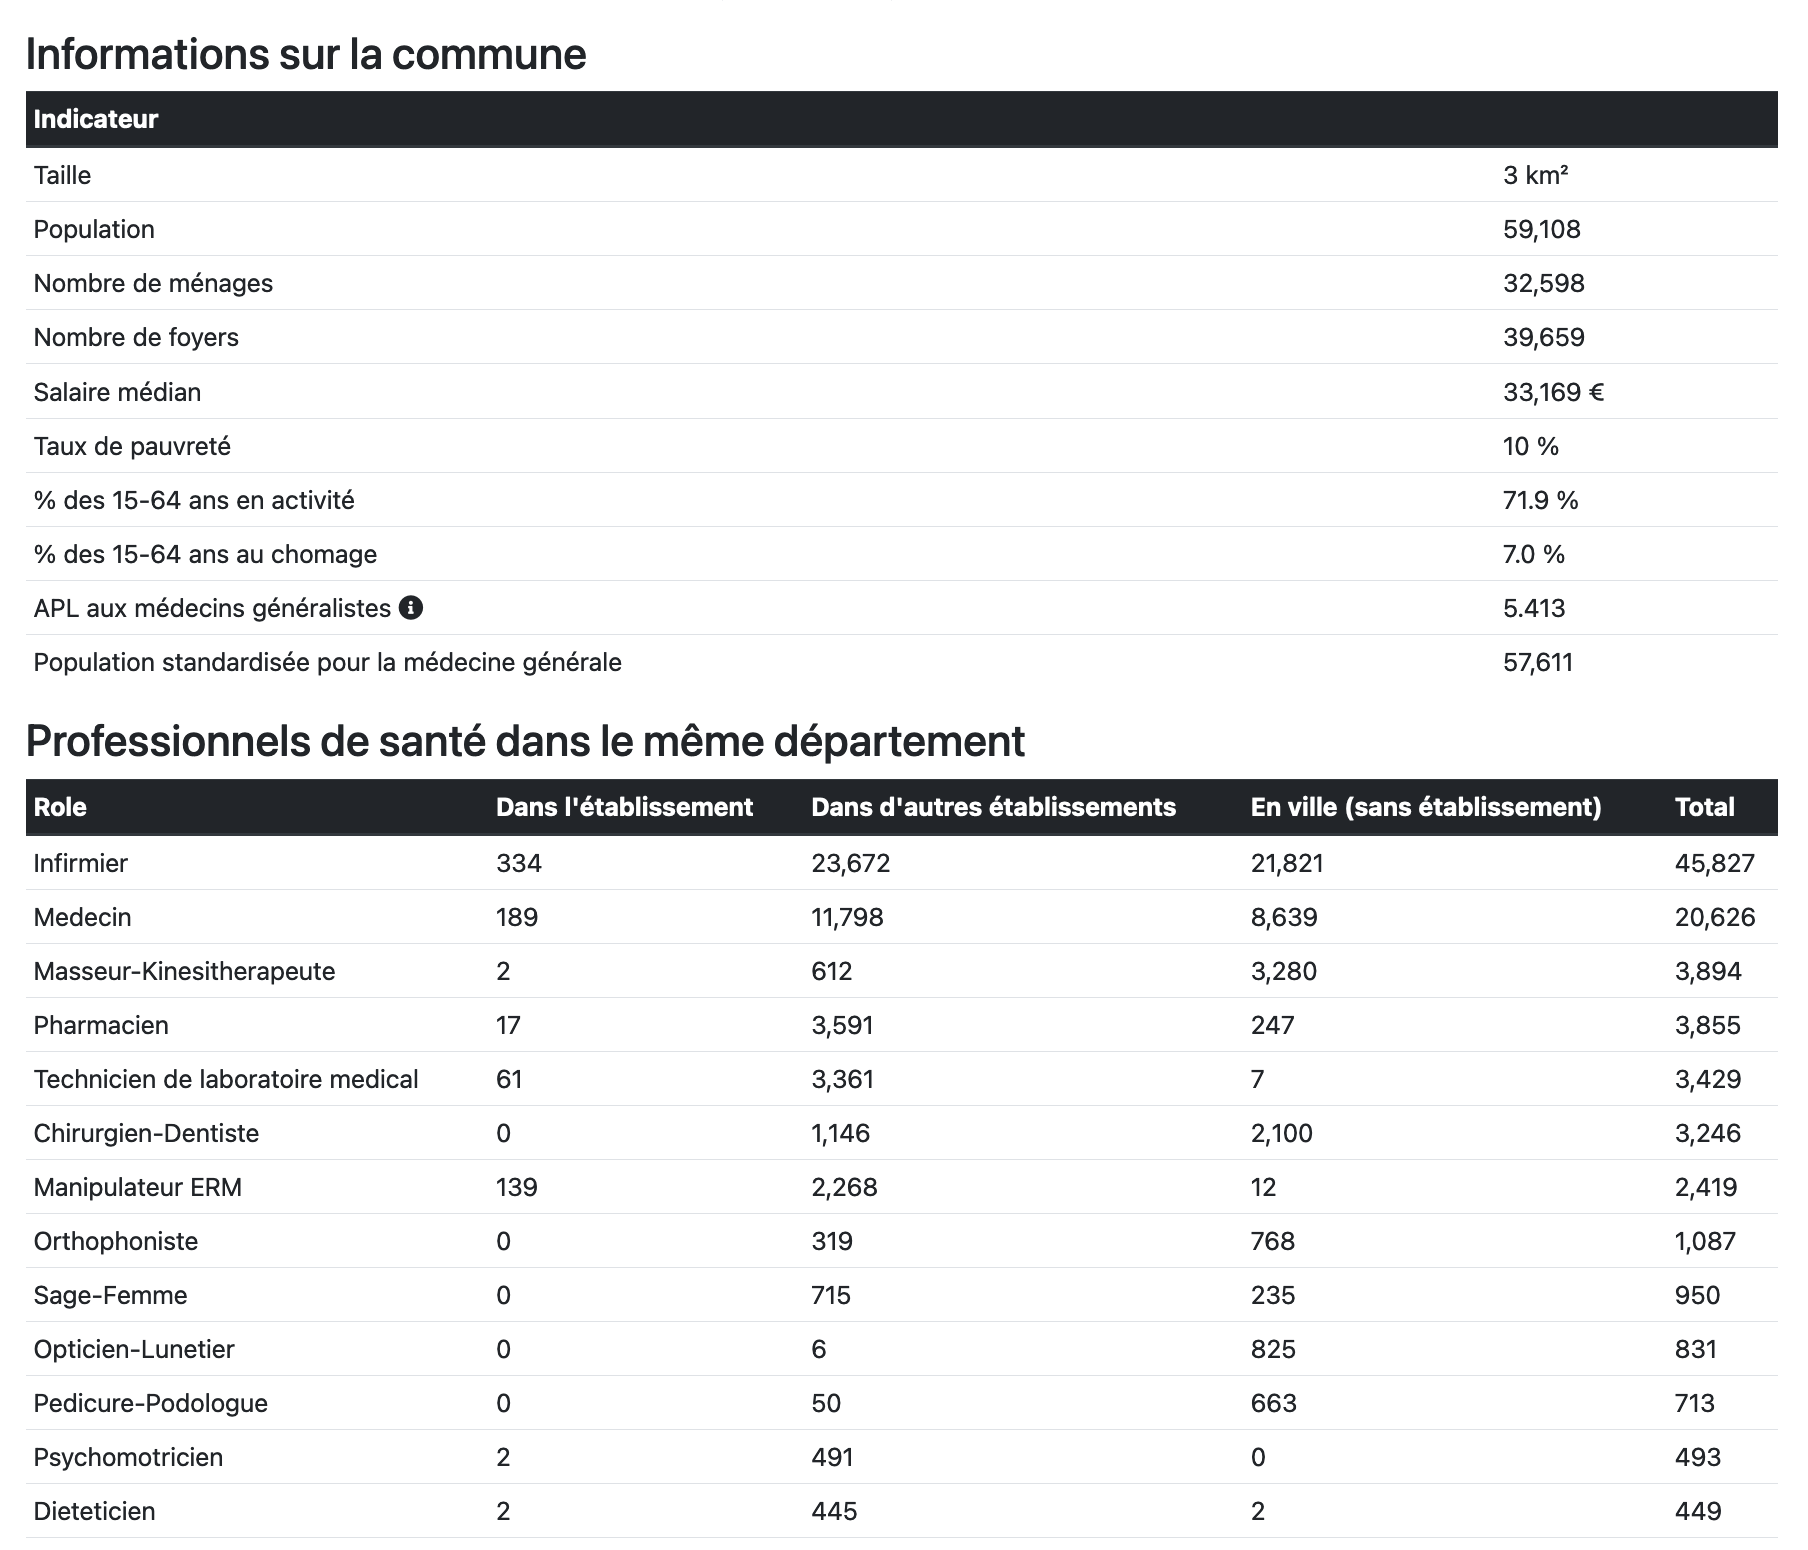
\includegraphics[width=0.7\textwidth]{images/healthcare-network/curie-commune.png}
%     \centering
%     \caption{
%         \textbf{Healthcare-Network: statistics on the municipality where Institut Curie Paris is located (Paris 75105).} Population, median salary and accessibility to primary care are displayed to qualify the hospital neighborhood. Health professionals within the department are also listed to illustrate the health supply available around the hospital.
%     }
%     \label{fig:hn-curie-commune}
% \end{figure}
